%%%%%%%%%%%%%%%%%%%%%%%%%%%%%%%%%%%%%%%%%
% Programming/Coding Assignment
% LaTeX Template
%
% This template has been downloaded from:
% http://www.latextemplates.com
%
% Original author:
% Ted Pavlic (http://www.tedpavlic.com)
%
% Note:
% The \lipsum[#] commands throughout this template generate dummy text
% to fill the template out. These commands should all be removed when 
% writing assignment content.
%
% This template uses a Perl script as an example snippet of code, most other
% languages are also usable. Configure them in the "CODE INCLUSION 
% CONFIGURATION" section.
%
%%%%%%%%%%%%%%%%%%%%%%%%%%%%%%%%%%%%%%%%%

%----------------------------------------------------------------------------------------
%	PACKAGES AND OTHER DOCUMENT CONFIGURATIONS
%----------------------------------------------------------------------------------------

\documentclass{article}
\usepackage{amssymb,amsmath}
\usepackage{fancyhdr} % Required for custom headers
\usepackage{lastpage} % Required to determine the last page for the footer
\usepackage{extramarks} % Required for headers and footers
\usepackage[usenames,dvipsnames]{color} % Required for custom colors
\usepackage{graphicx} % Required to insert images
\usepackage{subcaption}
\usepackage{listings} % Required for insertion of code
\usepackage{courier} % Required for the courier font
\usepackage{lipsum} % Used for inserting dummy 'Lorem ipsum' text into the template

% Margins
\topmargin=-0.45in
\evensidemargin=0in
\oddsidemargin=0in
\textwidth=6.5in
\textheight=9.0in
\headsep=0.25in

\linespread{1.1} % Line spacing

% Set up the header and footer
\pagestyle{fancy}
\lhead{\hmwkAuthorName} % Top left header
\chead{\hmwkClass\ (\hmwkClassTime): \hmwkTitle} % Top center head
%\rhead{\firstxmark} % Top right header
\lfoot{\lastxmark} % Bottom left footer
\cfoot{} % Bottom center footer
\rfoot{Page\ \thepage\ of\ \protect\pageref{LastPage}} % Bottom right footer
\renewcommand\headrulewidth{0.4pt} % Size of the header rule
\renewcommand\footrulewidth{0.4pt} % Size of the footer rule

\setlength\parindent{0pt} % Removes all indentation from paragraphs

%----------------------------------------------------------------------------------------
%	CODE INCLUSION CONFIGURATION
%----------------------------------------------------------------------------------------

\definecolor{MyDarkGreen}{rgb}{0.0,0.4,0.0} % This is the color used for comments
\lstloadlanguages{Python} % Load Perl syntax for listings, for a list of other languages supported see: ftp://ftp.tex.ac.uk/tex-archive/macros/latex/contrib/listings/listings.pdf
\lstset{language=Python, % Use Perl in this example
        frame=single, % Single frame around code
        basicstyle=\small\ttfamily, % Use small true type font
        keywordstyle=[1]\color{Blue}\bf, % Perl functions bold and blue
        keywordstyle=[2]\color{Purple}, % Perl function arguments purple
        keywordstyle=[3]\color{Blue}\underbar, % Custom functions underlined and blue
        identifierstyle=, % Nothing special about identifiers                                         
        commentstyle=\usefont{T1}{pcr}{m}{sl}\color{MyDarkGreen}\small, % Comments small dark green courier font
        stringstyle=\color{Purple}, % Strings are purple
        showstringspaces=false, % Don't put marks in string spaces
        tabsize=5, % 5 spaces per tab
        %
        % Put standard Perl functions not included in the default language here
        morekeywords={rand},
        %
        % Put Perl function parameters here
        morekeywords=[2]{on, off, interp},
        %
        % Put user defined functions here
        morekeywords=[3]{test},
       	%
        morecomment=[l][\color{Blue}]{...}, % Line continuation (...) like blue comment
        numbers=left, % Line numbers on left
        firstnumber=1, % Line numbers start with line 1
        numberstyle=\tiny\color{Blue}, % Line numbers are blue and small
        stepnumber=5 % Line numbers go in steps of 5
}

% Creates a new command to include a perl script, the first parameter is the filename of the script (without .pl), the second parameter is the caption
\newcommand{\pythonscript}[2]{
\begin{itemize}
\item[]\lstinputlisting[caption=#2,label=#1]{#1.pl}
\end{itemize}
}

%----------------------------------------------------------------------------------------
%	DOCUMENT STRUCTURE COMMANDS
%	Skip this unless you know what you're doing
%----------------------------------------------------------------------------------------

% Header and footer for when a page split occurs within a problem environment
\newcommand{\enterProblemHeader}[1]{
%\nobreak\extramarks{#1}{#1 continued on next page\ldots}\nobreak
%\nobreak\extramarks{#1 (continued)}{#1 continued on next page\ldots}\nobreak
}

% Header and footer for when a page split occurs between problem environments
\newcommand{\exitProblemHeader}[1]{
%\nobreak\extramarks{#1 (continued)}{#1 continued on next page\ldots}\nobreak
%\nobreak\extramarks{#1}{}\nobreak
}

\setcounter{secnumdepth}{0} % Removes default section numbers
\newcounter{homeworkProblemCounter} % Creates a counter to keep track of the number of problems
\setcounter{homeworkProblemCounter}{0}

\newcommand{\homeworkProblemName}{}
\newenvironment{homeworkProblem}[1][Part \arabic{homeworkProblemCounter}]{ % Makes a new environment called homeworkProblem which takes 1 argument (custom name) but the default is "Problem #"
\stepcounter{homeworkProblemCounter} % Increase counter for number of problems
\renewcommand{\homeworkProblemName}{#1} % Assign \homeworkProblemName the name of the problem
\section{\homeworkProblemName} % Make a section in the document with the custom problem count
\enterProblemHeader{\homeworkProblemName} % Header and footer within the environment
}{
\exitProblemHeader{\homeworkProblemName} % Header and footer after the environment
}

\newcommand{\problemAnswer}[1]{ % Defines the problem answer command with the content as the only argument
\noindent\framebox[\columnwidth][c]{\begin{minipage}{0.98\columnwidth}#1\end{minipage}} % Makes the box around the problem answer and puts the content inside
}

\newcommand{\homeworkSectionName}{}
\newenvironment{homeworkSection}[1]{ % New environment for sections within homework problems, takes 1 argument - the name of the section
\renewcommand{\homeworkSectionName}{#1} % Assign \homeworkSectionName to the name of the section from the environment argument
\subsection{\homeworkSectionName} % Make a subsection with the custom name of the subsection
\enterProblemHeader{\homeworkProblemName\ [\homeworkSectionName]} % Header and footer within the environment
}{
\enterProblemHeader{\homeworkProblemName} % Header and footer after the environment
}

%----------------------------------------------------------------------------------------
%	NAME AND CLASS SECTION
%----------------------------------------------------------------------------------------

\newcommand{\hmwkTitle}{Project\ \#4} % Assignment title
\newcommand{\hmwkDueDate}{April\ 4,\ 2017} % Due date
\newcommand{\hmwkClass}{CSC411} % Course/class
\newcommand{\hmwkClassTime}{L2501} % Class/lecture time
\newcommand{\hmwkAuthorName}{Angus Fung, Oleg Milyutin} % Your name

%----------------------------------------------------------------------------------------
%	TITLE PAGE
%----------------------------------------------------------------------------------------

\title{
\vspace{2in}
\textmd{\textbf{\hmwkClass:\ \hmwkTitle}}\\
\normalsize\vspace{0.1in}\small{Due\ on\ \hmwkDueDate}\\
\vspace{0.1in}
\vspace{3in}
}

\author{\textbf{\hmwkAuthorName}}
%\date{} % Insert date here if you want it to appear below your name

%----------------------------------------------------------------------------------------

\begin{document}

\maketitle
\clearpage
%----------------------------------------------------------------------------------------
%	PROBLEM 1
%----------------------------------------------------------------------------------------

% To have just one problem per page, simply put a \clearpage after each problem

\begin{homeworkProblem}
The following is the pseudocode on pg. 271 of Sutton and Barto:

\begin{figure*}[!ht]
\centering
\begin{subfigure}{\textwidth}
  \includegraphics[width=\linewidth]{policy.PNG}
  \centering
  \label{fig11}
\end{subfigure}
\caption{Reinforce}
\label{fig:11}
\end{figure*}

The Gaussian Policy is generated on line 91:
\begin{verbatim}
    pi = tf.contrib.distributions.Normal(mus, sigmas, name='pi')
\end{verbatim}

Mathematically, $\pi (a|s,\boldsymbol{\theta}) \sim N(\mu, \sigma^2)$, where $\mu$ is a fully-connected output (with tanh activation) of the neural network; and $\sigma^2$ is a bounded (above and below) fully-connected output with softplus activation. In the subsequent line (92):

\begin{verbatim}
    pi_sample = tf.tanh(pi.sample(), name='pi_sample')
\end{verbatim}

we sample from the distribution for actions $A_t$ that we \textit{actually} take (of course, this computation doesn't actually happen until later when \verb|sess.run| is executed). Since $\mu$ and $\sigma^2$ are outputs of the neural network, then $\pi$ contains 24 Gaussian distributions -- one for each type of action. \\\

Before optimization can happen, an episode $S_0, A_0, R_1,..., S_{T-1}, A_{T-1}, R_T$ needs to be generated. At the beginning of each episode, the initial parameters are reset; these are our initial state \verb|obs|, which represents our state. The sequences are generated within the while-loop starting on line 116. As mentioned earlier, the action depends on both our state $s$ and our weights (+bias) $\theta$. Line 119 picks this action by running our computational graph, feeding our current state \verb|obs|, and executing \verb|pi_sample|. \verb|pi_sample| is a tensorflow operation that samples from the normal distribution $\pi$ (where $\pi$ recall is an output of the neural network parametrized by $\theta$) and applying the tanh activation function. Once an action is picked, it is passed into the \verb|env.step| function which returns \verb|obs, reward, done, info|. \verb|obs| returns our new state through our last action, along with its associated reward \verb|reward|; \verb|done| is true if and only if the episode has terminated (e.g when the walker falls). The rewards are discounted by $\gamma=0.98$, where the more steps that are taken, the more the rewards at a particular step is discounted. All these sequences of values $\{S\}, \{A\}, \{R\}$ are stored in a list.\\\

Following sequence generation for a \textit{particular episode}, \verb|returns| is calculated in line 131. \verb|returns| calculates $G=[G_0, G_1, ...,G_T]$, the actual total reward from following policy $\pi$. Note that this is computed by subtracting the cumulative reward (which is monotonically increasing) from the total reward $G$. This results in a monotonically decreasing array, which makes sense -- after each step, we've taken a reward, so our expected reward from following policy $\pi$ all the way until the end is smaller. e.g if the total reward is $45$ at $G_0$, and the reward from $G_0$ to $G_1$ through action $A_0$ is 1, then our expected reward at $G_1$ is $44$.

After providing $G$, having both $\alpha$ and $\gamma$, all that's left is training (line 135), by passing as inputs the sequence of states $S$, $A$, and $G$ into the computational graph \verb|train_op|, defined on line 97:

\begin{verbatim}
    train_op = optimizer.minimize(-1.0 * Returns * log_pi)
\end{verbatim}

\verb|Returns| corresponds to $G_t$, and minimizing -\verb|log_pi| is equivalent to maximizing $\triangledown_{\theta}\log \pi(A_t|S_t,\theta)$ in the REINFORCE pseudocode. The updating of the weights (and bias) $\theta$ is handled with the \verb|optimizer| operation on line 96 wherein we pass the parameter $\alpha$.\\

After obtaining our updated $\theta$, a new episode (and its associated sequences $S, A, R$) are generated using it and the procedure continues \textit{ad infinitum} (or until a stopping condition). 


\end{homeworkProblem}
\begin{homeworkProblem}

Modifications:

\begin{enumerate}
    \item The gym environment was created:
    \begin{verbatim}
        env = gym.make('CartPole-v0')
    \end{verbatim}
    \item The number of outputs of the neural network was changed to two. 
    \begin{verbatim}
        hidden_size = 2
    \end{verbatim}
    This change corresponds to the two possible actions of cartpole: push to the left, or push to the right. 
    \item $\alpha$ was changed.
    \begin{verbatim}
        alpha = 0.0001 
    \end{verbatim}
    Learning rate -- empirically chosen based on performance. 
    \item $\gamma$ changed due to instruction specification:
    \begin{verbatim}
        gamma = 0.99 
    \end{verbatim}
    \item Changed the output placeholder to hold int32:
    \begin{verbatim}
        y = tf.placeholder(tf.int32, shape=(None, output_units), name='y')
    \end{verbatim}
    This is because $y$ corresponds to the discrete actions taken, which is either left (0) or right (1).
    \item Removed all other hidden layers and replaced it with this:
    \begin{verbatim}
        hidden = fully_connected( 
            inputs=x,
            num_outputs=hidden_size,
            activation_fn=tf.nn.softmax,
            weights_initializer=hw_init,
            weights_regularizer=None,
            biases_initializer=hb_init,
            scope='hidden')
    \end{verbatim}
    This is essentially a fully-connected neural network with two outputs, between $0$ and $1$ due to the softmax. This outputs correspond to probabilities $p$ and $1-p$ where $p$ is the probability of action $a=1$ and $1-p$ is the probability of action $a=0$.
    \item Changed the distribution to Bernoulli:
    \begin{verbatim}
        pi = tf.contrib.distributions.Bernoulli(p=hidden, name='pi')
    \end{verbatim}
    The above line will \textit{sample} from the distribution for two actions, one with probability $p$ and the other with probability $1-p$. Since we're only interested in the action based on $p$, we will discard the other action later.  
    \item Discard the other action:
    \begin{verbatim}
        obs, reward, done, info = env.step(action[0]))
    \end{verbatim}
    As mentioned earlier, we take only the first action corresponding to $p=1$.
    
    
    
\end{enumerate}


\end{homeworkProblem}

\clearpage


\begin{homeworkProblem}[Part 3a]
The following page shows the printout of the average number of steps and weights for the first 4000 episodes, in increments of 100. An $\alpha$ value of $0.0001$ through trial and error. Below is a plot displaying the number of \textbf{steps} and \textbf{mean steps} over the number of \textbf{episodes}. The number of mean steps was chosen to be the mean over 25 episodes. There are 8 weights, but as will be explained later, only 4 were displayed in the printouts as they are the weights that correspond to \verb|action [0]|. The significance and meaning of the weights are explained in part 3b.

\begin{figure*}[!ht]
\centering
\begin{subfigure}{\textwidth}
  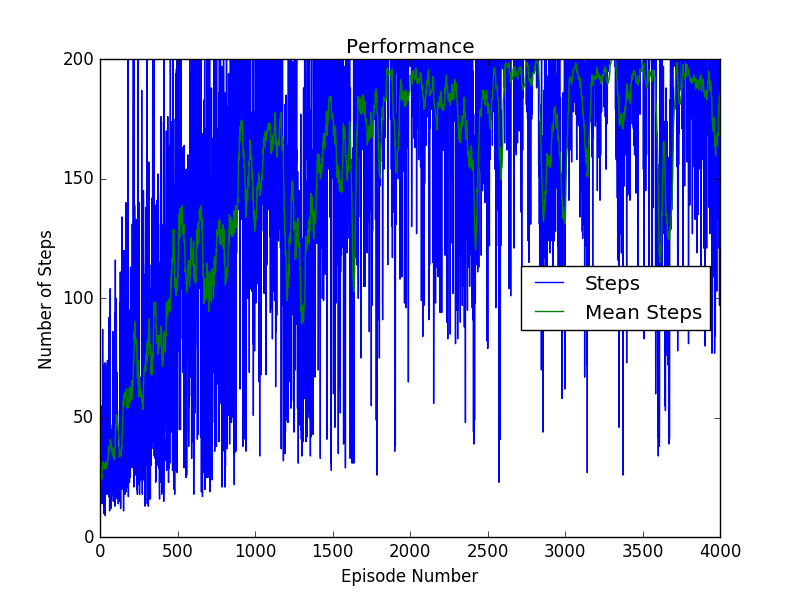
\includegraphics[width=\linewidth]{cartpole_mean.png}
  \centering
  \label{fig31}
\end{subfigure}
\caption{Steps per Episode}
\label{fig:31}
\end{figure*}

\begin{figure*}[!ht]
\centering
\begin{subfigure}{\textwidth}
  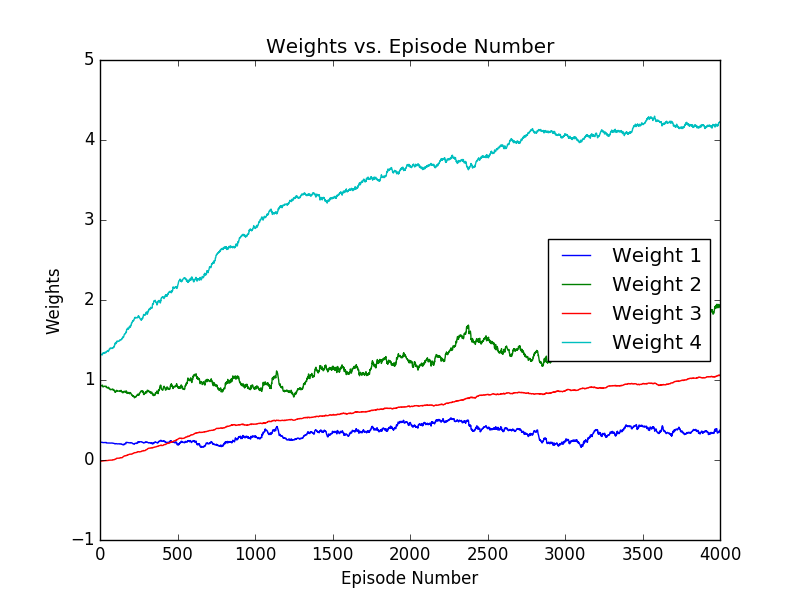
\includegraphics[width=\linewidth]{cartpole_weights.png}
  \centering
  \label{fig32}
\end{subfigure}
\caption{Weights per Episode}
\label{fig:32}
\end{figure*}

\clearpage
\begin{verbatim}
Episode 0 finished after 16 steps with return 14.854222890512432
Average number of steps over the last 25 episode is 16.0
incoming weights: [ 0.22191776  0.93468541 -0.01397642  1.31265676]
Episode 100 finished after 75 steps with return 52.941335841434956
Average number of steps over the last 25 episode is 45.84
incoming weights: [ 0.20439152  0.85509539  0.01344092  1.46339333]
Episode 200 finished after 37 steps with return 31.055091413092182
Average number of steps over the last 25 episode is 60.16
incoming weights: [ 0.21634713  0.83159864  0.0719261   1.68246746]
Episode 300 finished after 117 steps with return 69.14555293653483
Average number of steps over the last 25 episode is 74.64
incoming weights: [ 0.22342783  0.84006906  0.12938082  1.84264755]
Episode 400 finished after 119 steps with return 69.75955643309779
Average number of steps over the last 25 episode is 77.64
incoming weights: [ 0.23595828  0.8809585   0.18039189  2.03197455]
Episode 500 finished after 134 steps with return 73.99145386222733
Average number of steps over the last 25 episode is 108.12
incoming weights: [ 0.196678    0.92328918  0.25714341  2.16532993]
Episode 600 finished after 106 steps with return 65.53878166524818
Average number of steps over the last 25 episode is 115.88
incoming weights: [ 0.24281117  1.04575861  0.31841072  2.25216007]
Episode 700 finished after 144 steps with return 76.4783370759589
Average number of steps over the last 25 episode is 98.4
incoming weights: [ 0.20235683  0.99107575  0.36334991  2.36789417]
Episode 800 finished after 36 steps with return 30.358678195042607
Average number of steps over the last 25 episode is 125.52
incoming weights: [ 0.20740327  0.89683598  0.40363207  2.6555233 ]
Episode 900 finished after 200 steps with return 86.6020325142037
Average number of steps over the last 25 episode is 167.72
incoming weights: [ 0.29155162  0.98207104  0.44190452  2.77825546]
Episode 1000 finished after 139 steps with return 75.26613141061311
Average number of steps over the last 25 episode is 130.4
incoming weights: [ 0.29265186  0.90145683  0.4489117   2.89901829]
Episode 1100 finished after 162 steps with return 80.37084859769736
Average number of steps over the last 25 episode is 165.32
incoming weights: [ 0.32957476  0.91997194  0.48202854  3.12034416]
Episode 1200 finished after 137 steps with return 74.76393369106532
Average number of steps over the last 25 episode is 115.88
incoming weights: [ 0.26277456  0.8672111   0.49845141  3.1980412 ]
Episode 1300 finished after 47 steps with return 37.64746051087996
Average number of steps over the last 25 episode is 89.6
incoming weights: [ 0.27406445  0.89333415  0.5170083   3.31030273]
Episode 1400 finished after 167 steps with return 81.33287232842956
Average number of steps over the last 25 episode is 156.84
incoming weights: [ 0.36245888  1.1207422   0.54691505  3.32228947]
Episode 1500 finished after 200 steps with return 86.6020325142037
Average number of steps over the last 25 episode is 176.32
incoming weights: [ 0.35379398  1.1633296   0.56380141  3.26984262]
Episode 1600 finished after 200 steps with return 86.6020325142037
Average number of steps over the last 25 episode is 155.92
incoming weights: [ 0.30168197  1.07839549  0.57944453  3.35927129]
Episode 1700 finished after 200 steps with return 86.6020325142037
Average number of steps over the last 25 episode is 184.92
incoming weights: [ 0.36993358  1.07966614  0.60298175  3.50889945]
Episode 1800 finished after 200 steps with return 86.6020325142037
Average number of steps over the last 25 episode is 154.24
incoming weights: [ 0.35088313  1.21788228  0.63187838  3.50044322]
Episode 1900 finished after 189 steps with return 85.0358594396383
Average number of steps over the last 25 episode is 173.0
incoming weights: [ 0.39665371  1.17079353  0.64570022  3.62058377]
Episode 2000 finished after 200 steps with return 86.6020325142037
Average number of steps over the last 25 episode is 193.12
incoming weights: [ 0.46253765  1.2161032   0.66628808  3.6823895 ]
Episode 2100 finished after 200 steps with return 86.6020325142037
Average number of steps over the last 25 episode is 184.32
incoming weights: [ 0.44863737  1.24216187  0.68448853  3.65436864]
Episode 2200 finished after 102 steps with return 64.12517023181074
Average number of steps over the last 25 episode is 181.96
incoming weights: [ 0.47226307  1.2361778   0.69206059  3.75535107]
Episode 2300 finished after 200 steps with return 86.6020325142037
Average number of steps over the last 25 episode is 185.16
incoming weights: [ 0.48462847  1.4766072   0.73599935  3.72774601]
Episode 2400 finished after 105 steps with return 65.19068855075574
Average number of steps over the last 25 episode is 156.24
incoming weights: [ 0.37560239  1.47521901  0.77768552  3.68007207]
Episode 2500 finished after 200 steps with return 86.6020325142037
Average number of steps over the last 25 episode is 181.32
incoming weights: [ 0.39237449  1.52184308  0.82061023  3.78122568]
Episode 2600 finished after 200 steps with return 86.6020325142037
Average number of steps over the last 25 episode is 179.4
incoming weights: [ 0.36007991  1.32962692  0.82774675  3.92799187]
Episode 2700 finished after 200 steps with return 86.6020325142037
Average number of steps over the last 25 episode is 194.96
incoming weights: [ 0.38800335  1.4183327   0.84438801  3.96517777]
Episode 2800 finished after 200 steps with return 86.6020325142037
Average number of steps over the last 25 episode is 194.36
incoming weights: [ 0.35733446  1.30751836  0.82287872  4.10220909]
Episode 2900 finished after 167 steps with return 81.33287232842956
Average number of steps over the last 25 episode is 159.4
incoming weights: [ 0.20434627  1.22068048  0.83585072  4.10004759]
Episode 3000 finished after 155 steps with return 78.94015538032704
Average number of steps over the last 25 episode is 133.16
incoming weights: [ 0.2359065   1.33660197  0.86128759  4.06835556]
Episode 3100 finished after 200 steps with return 86.6020325142037
Average number of steps over the last 25 episode is 191.16
incoming weights: [ 0.17258523  1.43373084  0.89118266  3.99433637]
Episode 3200 finished after 184 steps with return 84.26467178922091
Average number of steps over the last 25 episode is 192.76
incoming weights: [ 0.38062871  1.54989552  0.90226227  4.07167864]
Episode 3300 finished after 200 steps with return 86.6020325142037
Average number of steps over the last 25 episode is 199.72
incoming weights: [ 0.34398791  1.4805975   0.92580551  4.1234479 ]
Episode 3400 finished after 200 steps with return 86.6020325142037
Average number of steps over the last 25 episode is 188.04
incoming weights: [ 0.42376432  1.64179933  0.94751042  4.08511925]
Episode 3500 finished after 200 steps with return 86.6020325142037
Average number of steps over the last 25 episode is 199.08
incoming weights: [ 0.42080951  1.59644723  0.95429921  4.20116615]
Episode 3600 finished after 119 steps with return 69.75955643309779
Average number of steps over the last 25 episode is 147.2
incoming weights: [ 0.34576482  1.38984323  0.93738985  4.2435894 ]
Episode 3700 finished after 200 steps with return 86.6020325142037
Average number of steps over the last 25 episode is 173.8
incoming weights: [ 0.35796618  1.62665439  0.97434902  4.17556047]
Episode 3800 finished after 200 steps with return 86.6020325142037
Average number of steps over the last 25 episode is 193.48
incoming weights: [ 0.34360367  1.75089157  1.01845813  4.17612362]
Episode 3900 finished after 200 steps with return 86.6020325142037
Average number of steps over the last 25 episode is 185.12
incoming weights: [ 0.35249045  1.86527658  1.02694583  4.15076399]
\end{verbatim}
\end{homeworkProblem}
\clearpage

\begin{homeworkProblem}[Part 3b]
The final weights, over 4000 episodes, is:
\begin{verbatim}
[[ 0.35249045  1.03760803]
 [ 1.86527658 -0.96739352]
 [ 1.02694583 -0.80850083]
 [ 4.15076399 -2.54075646]]    
\end{verbatim}

The 2-tuple represents the weights going to the $p$ output and $1-p$ output, respectively. Since we considered only the output corresponding to $p$ (\verb|action[0]|), only the first of each tuple will be analyzed. From the source code, the four inputs correspond are $x$, $\dot{x}$, $\theta$ and $\dot \theta$, which are the cart position, cart velocity, pole angle, and angular velocity of the pole, respectively. Their corresponding weights are $w_x=0.35, w_v=1.87, w_{\theta}=1.03, w_w=4.15$. Therefore, our output is $p=\text{softmax}(x w_x + v w_v + \theta w_{\theta} + w w_w)$. Instead of analyzing that expression in terms of a probability, it is more insightful to think in terms of the \textit{objective} that maximizes the reward: it in fact serves as a \textit{controller}.\\

By a controller, it is analogous to a \textit{proportional controller} in control theory. That is, when the pole is falling close to the 15 degree threshold and its state $s$ is fed back into the input of the neural network, the output should act in such a way that the pole moves in the \textit{opposite} direction. Therefore, it makes sense to draw a parallel with this in terms of a linear control force.\\

From a qualitative analysis, it is clear that the weights should be positive, which is the case here. Consider a simple scenario wherein the cart is at the centre of the track, stationary, with the pole at an angle and no angular velocity. A positive value of $w_{\theta}$ will provide a force that pushes the pole back to the centre. Similarly, a positive value of $w_{w}$ will reduce the angular velocity.\\

Suppose the cart is on the right side of the track, then we'd expect the neural network to act in such a way to push the cart back to the centre. It does this, but indirectly. The positive weight of $w_x$ will cause the cart to move further to the right, which in tern causes the pole to move to the left. As the angle $\theta$ becomes more and more negative, that causes the cart to move to left towards the centre.\\

Finally, a positive weight for $w_v$ makes sense -- consider a scenario where the pole is perfectly balanced, and the cart accelerating to the right. The dominant term in the output $w_v$ will cause the cart to accelerate more to the right. While seemingly contradictory, this causes the pole to fall left (negative angle), and thus the increasingly large negative term will cause a net effect of reducing the cart's velocity.\\

Thus $w_{\theta}$ and $w_w$ act to bring the pole to its upright position, and $w_x$ and $w_v$ act to regulate the cart to the centre. The magnitudes of the weights determine the neural network's priority. The large weight corresponding to $w_w$ could mean the neural network is particular sensitive to changes in angular velocity. Seeing as the pole has to be within 15 degrees of its upright position, that would make sense. 


\end{homeworkProblem}
\end{document}